\documentclass{article}
\usepackage{amssymb}
\usepackage{amsfonts}
\usepackage{amsmath}
\usepackage{cancel}
\usepackage{graphicx}
\graphicspath{ {./assets/} }
\author{Enlai Li}
\title{MATH240 \textendash{} Lecture 2}
\date{January 6, 2023}
\begin{document}
\maketitle
\section{Set algebra}
When are sets equal? For instance:
\begin{align*}
    A & = \{x \in \mathbb{Z} \ | \ x=2k-1 \text{ for some } k \in \mathbb{Z}\} \\
    B & = \{x \in \mathbb{Z} \ | \ x=2n+1 \text{ for some } n \in \mathbb{Z}\}
\end{align*}
We need to prove:
\begin{enumerate}
    \item $A \in B$
    \item $B \in A$
\end{enumerate}
1. NTS (need to show): if $x \in A$ then $x \in B$
\begin{gather*}
    \text{Assume } x \in A \text{ so } x = 2k-1 \text{ for some }k\in \mathbb{Z}
    = 2k-2+2-1
    =2(k-1)+1  \\
    \text{With }n=k-1 \text{ we have }x=2n+1 \\ \text{ therefore } A=B
\end{gather*}
2. $x \in B \Rightarrow x\in A$
Let $x=2n+1 \text{ where } n\in \mathbb{Z}$, then
\begin{align*}
    x & =2n+2-2+1 \\
      & =2(n+1)-1
\end{align*}
If $k=n+1$ then $x=2k-1 \Rightarrow x\in A$

\section{Set operations}

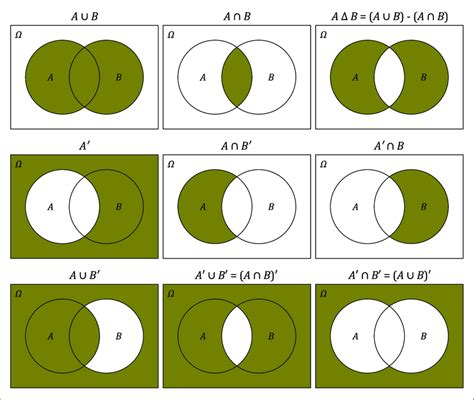
\includegraphics[width=\textwidth]{l1_venn_ab}
$U =$ The universe of objects
\begin{itemize}
    \item Union
          \[
              A \cup B =\{x\in U \ | \ x \in A \text{ or } x \in B\}
          \]
    \item Intersection
          \[
              A \cap B = \{x \in U \ | \ x \in A \text{ and } x \in B\}
          \]
    \item Difference
          \[
              A \backslash B = A-B = \{x \in A \ | \ x \notin B\}
          \]
    \item Complement \[
              \overline{A} = A' = \{x \in U \ | \ x \notin A\} = U \backslash A
          \]ex:
          \begin{align*}
              A            & = \{1,2,3\}      \\
              U            & = \mathbb{N}     \\
              \overline{A} & =\{0,4,5,\dots\}
          \end{align*}
    \item Symmetric Difference \begin{align*}
              A \oplus B & = \{x \in U \ | \ x \in A \text{ or } x \in B \text{ , but not both } \} \\
                         & = (A \backslash B) \cup (B \backslash A)                                 \\
                         & = (A\cup B) \backslash (A \cap B)                                        \\
                         & = (A\cup B) \cap (A\cup B)
          \end{align*}
          ex:
          \begin{align*}
              A          & = \{1,2,3\}   \\
              B          & = \{3,4,5\}   \\
              A \oplus B & = \{1,2,4,5\}
          \end{align*}


\end{itemize}
\section{Set identities}
Theorem: If two sets A and B have the same Venn diagram, then $A=B$
\\ Proof: We need to show $A \subseteq B \text{ and } B \subseteq A $ (They have similar proof)
\begin{enumerate}
    \item $A \subseteq B$ \\ Let $x \in A$, then x is in the shaded region of A's Venn diagram. So it's also in shaded version of B's Venn diagram, so $x \in B$
    \item $B \subseteq A$ \\ Let $x \in B$, then x is in A's region. So it's also in B's region, so $x \in A$
          \\ \hspace*{\fill} $\square$

\end{enumerate}

\subsection{Laws of boolean algebra}
\marginpar[]{\raggedright{} Laws of boolean algebra are complete set of rules}
\begin{itemize}
    \item Identify law: \begin{align*}
              A \cup \emptyset & = A \\
              A \cap U         & = A
          \end{align*}
    \item Idempotent laws: \begin{align*}
              A \cup A & = A \\
              A \cap A & = A
          \end{align*}
    \item Domination laws: \begin{align*}
              A \cup U         & = U         \\
              A \cap \emptyset & = \emptyset
          \end{align*}
    \item Double complement laws: \[
              \overline{\overline{A}} = A
          \]
    \item Commutative laws: \begin{align*}
              A \cup B & = B \cup A \\
              A \cap B & = B \cap A
          \end{align*}
    \item Complement laws: \begin{align*}
              A \cup \overline{A} & = U         \\
              A\cap \overline{A}  & = \emptyset
          \end{align*}
    \item Associative laws: \begin{align*}
              (A\cup B)\cup C & = A\cup(B\cup C)
              \\(A\cap B)\cap C & = A\cap(B\cap C)
          \end{align*}
    \item Distributive laws: \begin{align*}
              A\cup (B\cap C) & = (A\cup B)\cap(A\cup C)
              \\A\cap(B\cup C)& = (A\cap B)\cup(A\cap C)
          \end{align*}
    \item De Morgan's law: \begin{align*}
              \overline{A \cup  B} & = \overline{A}\cap \overline{B}  \\
              \overline{A \cap B}  & = \overline{A}\cup  \overline{B}
          \end{align*}
    \item Absorption law: \begin{align*}
              A \cup (A \cap B) & = A \\
              A \cap (A \cup B) & = A
          \end{align*}
          \marginpar[]{\raggedright{} Note: Past 3 sets or more than 2 levels of set equations, Venn diagrams become impossible to read But we can use the laws of boolean algebra to derive new set identities algebraically.}
\end{itemize}
ex: Check $A \cup (B \cap C) = (A \cup B) \cap (A \cup C)$

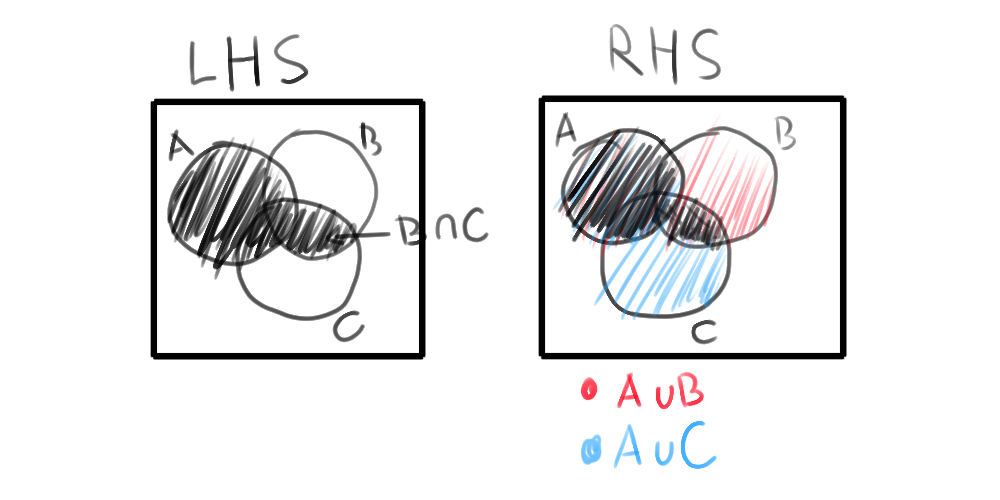
\includegraphics{l2_2}

ex: use set laws to show
\[
    \overline{A \cup (B \cap C)} = (\overline{C}\cup \overline{B})\cap \overline{A}
\]
\begin{align*}
    \overline{A \cup (B \cap C)} & = \overline{A} \cup \overline{(B \cup C)} \text{ (De Morgan) }               \\
                                 & = \overline{A} \cup (\overline{B}\cap \overline{C}) \text{ (De Morgan) }     \\
                                 & = \overline{A} \cup (\overline{C}\cap \overline{B}) \text{ (Commutativity) } \\
                                 & = (\overline{C}\cap \overline{B}) \cup \overline{A} \text{ (Commutativity) }
\end{align*}

\subsection{External set operations}
The following set operations change the universe of the set
\begin{itemize}
    \item Cartesian product: $A \times B = \{(a,b) \ | \ a\in A, b\in B\}$ \text{ (set of ordered pairs) }\\
          \marginpar[]{\raggedright{} Cardinality: $\lvert A \times B \rvert = \lvert A \rvert \times  \lvert B \rvert $}
          ex: \begin{gather*}
              A = \{1,2,3\} \quad B = \{0,1\} \\
              A \times B = \{(1,0), (2,0),(3,0),(1,1)(2,1)(3,1)\}
          \end{gather*}
          ex2: \[
              \{(x,y)\ \vert \ x\in \mathbb{R} , y \in \mathbb{R} \} = \mathbb{R} \times \mathbb{R} = \mathbb{R} ^{2} \text{ (The set of 2-dimensional vectors)}
          \]
    \item Power set: $\{x \ \vert \ x \subseteq A\}$ \text{ (set of all subsets)}
          \marginpar[]{\raggedright{} Cardinality: $\lvert P(A) \rvert = 2 ^{\lvert A \rvert }$}
          ex: \begin{align*}
              A    & = \{1,2,3\}                                                                                   \\
              P(A) & = \{\emptyset , \{1\}, \{2\}, \{3\}, \{1,2\}, \{2,3\},\{1,3\},\{1,2,3\}\}\text{ (8 elements)} \\
          \end{align*}
          ex2: \begin{gather*}
              P(\emptyset ) = \{\emptyset \} \text{ (1 element)} \\
              \lvert P(\emptyset ) \rvert = 1
          \end{gather*}
\end{itemize}



\end{document}